\chapter{寻找改进机会} % Introduction chapter suppressed from the table of contents

客户：想改善我们的敏捷开发过程，但没有概念应该怎么开始？\\
我：可以借用评估，例如CMMI评估。\\
客户：CMMI不是和敏捷打对台吗？\\
我：这是很多人的误解，把CMMI等同于瀑布式开发，而且误认为CMMI评估只是认证(类似ISO认证）。本来CMMI的目的是帮助企业，例如美国国防部，评价自己和供应商的软件开发过程质量、诊断软件工程软件开发过程有哪些不足。所以CMMI
很全面地覆盖项目管理、软件工程等领域。

敏捷过程，例如 SCRUM、 XP
等都能对上大部分的CMMI实践。但反过来敏捷的实践只包括部分CMMI实践，不全面，例如缺少组织级部分，最新的V2.0
版本更精简，更适合敏捷团队。\\

客户：怎么可以利用CMMI？学习一下资料就可以了吗？\\
我：这也是很多团队的误解，跟培训学习的道理一样，若只是吸收了知识，没动手动脑筋，不会有什么作用。我刚开始做CMMI评估时，有些企业说：”CMMI是挺好的，但我们不需要花这么多钱、精力去做评估，平时按照你发的模型与参考材料，学习一下就可以了，我们团队学习力很强。“但过了6个月、或一两年后，再次拜访客户，99%概率一点改进都没有。所以评估本身就是改进的驱动力、再配合评估，作为过程改进的里程碑，使团队有集中改善的压力。你可以想象如果没有评估的话，大家都忙，哪里会有时间与动力回顾并改善平常于平常习惯了的做法。（可参考附件案例，了解CMMI评估如何帮助项目组提升）\\

但请注意，虽然评估能帮我们识别出一些改进点，但过程改进必须做好相关纠正措施。\\
客户：请解释一下。\\
我：首先要理解纠正措施(Corrective Action) 和改正(Correction) 的区别。这一点我刚开始接触CMMI的时候，已经听过，但没有充分了解。\\


\begin{itemize}
\tightlist
\item
  改正Correction只是针对问题的表面，去处理，不能长期避免同类问题再发生。
\item
  纠正措施Corrective action
   是针对问题分析和发现背后的根本原因并制订对应改进计划。
\end{itemize}

很多时候团队仅仅利用问题跟踪表，把评估发现的问题一一解决，只做Correction，做事习惯没有变化，后面同类问题还是会重复出现。所以更应分析问题根因，并识别哪些改进项目会有效果，然后以项目方式立项做改进。\\
客户：你说的好像还是挺有道理，是否可以举些例子。\\
下面就举一个关于组织培训的实例。\\
==评估中访谈公司培训专员==
评估师：请问你们如何与上级和管理层汇报公司培训的情况？\\
培训专员：我们每次都有培训报告，内容包括学员的考试成绩、反馈、出席情况等。也有每年的总结报告，包括整年所有的培训，比如实际与计划对比、费用与预算比较等等。\\
我：是否可以举例？\\

培训专员：例如我们比较关注信息安全。因为很多客户尤其是政府客户也注重这一点，所以我们就找一些外面的培训课，专门对员工做一个线上的信息安全培训。大概有100个人参加，为了衡量培训效果，有考试题库，及格分数线是80分，但是第一轮考试只有60多位及格，我们觉得效果不好，要求那些不及格的重考。第二次还是有20位左右不通过。\\

评估师：你们觉得效果如何？满意吗？\\

培训专员：不太满意，但后面该怎么做呢？

\begin{description}
\item[]
\begin{description}
\tightlist
\item[]
。 。 。 。 。
\end{description}
\end{description}

评估师：请问你们如何培训新进公司的开发人员？\\
培训专员：我们都有一系列的新员工技术培训课，上午会讲一些原理要求，然后会有一些编码练习，比如如何设计跟开发一个人事管理系统。我们会把用的框架和复用组件放到内网，方便他们获取使用。也会定好系统的主要模块和相关的测试用例，让他们可以在编程的时候用上那些原则和理论。
评估师：挺好的，你们如何对他们做反馈？\\
培训专员：我作为老师会对他们的开发进行评价、打分，告知他们不足之处。\\
评估师：是指我们平常年终评价那种，按表现的优秀程度打分吗？\\
培训专员：差不多，我们会从不同的角度去评价。比如我们强调是否按公司的编码规程？是否满足面向对象不耦合原则？从多个角度去评价，进行综合打分。\\

\hypertarget{ux603bux7ed3ux8bbfux8c08ux7684ux95eeux9898ux53d1ux73b0}{%
\subsection{总结以上访谈的问题}\label{ux603bux7ed3ux8bbfux8c08ux7684ux95eeux9898ux53d1ux73b0}}

大家可以从以上访谈发现下面2问题，并针对每一条问题制定改正措施：

\begin{enumerate}
\tightlist
\item
  发现培训反馈靠主观，只是靠老师主观打分，可以加考试就可以满足不客观了
\item
  发现有些课学生成绩及格率低，下一次同类外部培训要求学员备课，以提高学生的通过率
\end{enumerate}

是采取这些行动，对公司级培训质量改进作用吗？ 几乎没有，因为只是对问题做correction,没有改变系统与习惯，类似问题还是会再出现。\\
几乎没有，因为只是对问题做correction,没有改变系统与习惯，类似问题再出现，还是以前的做法。\\
但如能深入探索根因，就发现原来新员工正式上课的培训不长，只有一天，大部分还是靠新员工在工作中，跟有经验``老''员工导师，老带新，边做边学。但因为很多有经验的都忙于做项目，没有时间带领新员工，所以主要依赖新员工自学，导致新员工培训的效果差异很大。\\
也正因为员工都没有持续学习的习惯，都是边做边学，参加比较正式的课程前都没有备课的习惯，导致及格率比较低。也发现原来公司有给客户开发并提供线上学习平台。\\
评估师问：为什么没有类似的内部平台用于内部培训？\\
公司总监：平台我们是有的，但是没有课件。我们工作也很独特，没有一些可以买回来的培训可以用。所以一直都没有计划用这个平台。\\
评估师：现在很多公司，尤其疫情原因，都倾向利用培训平台帮助员工学习，虽然没有传统面对面的培训效果好，但肯定会比自学好多了，同时还有上课记录、考试等度量。但须要公司花时间、精力去准备课件，才对公司级培训有作用。\\
后面总监在评估后，与大家讨论这个评估的发现，大家都同意这做法会有帮助，并且评价这个改进项目的投入和价值，最终成功立项，作为下半年的主要改进项目之一。\\
%客户：听完你这个例子，回顾一下我们每年都会有各种评估，但只是针对每一个发现的问题做一些修正，确实对整个公司的质量没有任何提升的作用。大家做事的习惯还是一样，把评估和处理问题当成一些常规性应付的工作。

%\href{文件:IssuesScreenshot_2022-10-19_205655.jpg}{600px}

%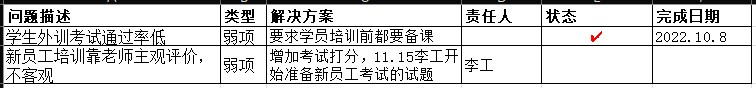
\includegraphics[width=10cm]{IssuesScreenshot_2022-10-19_205655.jpg}

客户：回顾我们每年都会有各种评估，但评估后只是针对发现的问题做修正，对整个公司的质量确实没有任何提升的作用。大家做事的习惯还是一样，把评估和处理问题当成一些常规性应付的工作。\\

我：所以要质量改进，必须针对弱点找出根因，并有相关改进项目才有效果。如果希望利用评估做改进，首先大家的心态要改过来，如果只追求通过评估的心态，只给评估组看最好的一面，不让问题暴露，对公司的质量改进没有作用。但是反过来，如果大家希望这些模型能帮助发现不足，识别改进的机会，评估可以很全面地帮助我们，就好像去医院做体检一样，各方面都会帮我们看。所以每次评估时，我都会让大家放心，千万不要担心问题被发现，我们发现的问题都不是个人或者项目组的问题，都是系统的问题，系统有不足，才导致有这些问题发生。所以每次评估也必须遵守保密跟不追究原则，让大家可以放心说出不足，才可以起改进的作用。

\hypertarget{ux7ba1ux7406ux5c42ux7684ux7406ux89e3ux4e0eux652fux6301}{%
\subsection{管理层的理解与支持}\label{ux7ba1ux7406ux5c42ux7684ux7406ux89e3ux4e0eux652fux6301}}

评估发现会分成弱项与建议两类：

\begin{itemize}
\tightlist
\item
  弱项是指跟模型的要求有明显差距
\item
  建议比弱项程度轻，没有明显差距但可以改善的点\\
\end{itemize}

评估过程要求标弱项必须要得到内部评估组成员认同。某次评估，某些内部评估组成员对弱项就特别担心，尽量想办法解释。有些弱项可能要反复讨论十几二十分钟，他们确实没办法才接受。

"我们理解你说项目量化管理计划模板中写公司基线的地方应该是公司目标，公司目标里应该是写总体的年度目标，我们同意模版有不足，应该后面改善，但应该算是建议，不能当成弱项。``

但是如果提的是建议，一点问题都没有。为什么发现弱项跟建议反应区分这么大呢？\\
后来发现，原来领导关注评估，看弱项多少，觉得如果弱项多就表示相关人没做到位，但恰恰是管理者这种心态妨碍了企业的过程改进，因为要改进，首先要觉得本身有不足，才有动力挖掘不足的根因并做改进。


\framebox{%
\begin{minipage}[t]{0.97\columnwidth}\raggedright
评估师问：您觉得你们配置管理做得如何？有没有一些你不满意的地方？\\
研发总监：挺好的。没有问题。\\
（但实际上，从文档检查已发现在配置审计、建立基线、基线变更、如何保证文档、环境配置与代码同步等都有不足。）
\strut
\end{minipage}}

所以如果想利用评估来做改进，首先管理者要觉得本身有不足，并理解评估的目的，就好比我们做代码走查，如果没发现是坏事一样道理。

如想多了解应如何分析根因，并在敏捷项目中使用，例如冲刺回顾，请看下部分。

\hypertarget{ux603bux7ed3}{%
\subsection{结束语}\label{ux603bux7ed3}}

CMMI 过程改进的成功要素：\\
\textbf{1.时间}
如果公司希望借用CMMI确实做到一些具体的改进，因为要足够的时间来累积数据，整个项目时间不能太短，比如小于6个月就很难达到改进效果。\\
\textbf{2.计划}
一开始就要做好计划，企业要有过程改进组人员的投入，包括负责度量与分析。而且还要有合适的工具，单靠手工很难收集真正的项目数据。\\
\textbf{3.方法}
培训不仅仅是教CMMI模型，更重要是有一些具体的方法、模板、工具，可以让项目组立马用起来。项目实战辅导很关键，听得懂并不一定会用，老师的实战辅导才能真正将方法落到实处。\\
\textbf{4.使用功能点估算项目规模使项目间可比}
直接从需求估算功能点数，让不同项目的度量数据可比，不然无法建立公司基线。\\
\textbf{5.工具与平台}
尽量用工具取代人手工作，例如，提供了从需求计算功能点数的模板工具等。\\
\textbf{6.高层的支持}
高层与事业部领导的支持非常重要，可以想象如果他们不认同这些对企业长远的帮助，很难要求他们投入这么多人力资源在这个项目中。
如果领导不关心，很可能评估过后便恢复到改进前的状态，不能持续。

\hypertarget{ux9644ux4ef6}{%
\section{附件}\label{ux9644ux4ef6}}

\hypertarget{cmmiux8bc4ux4f30ux6848ux4f8b}{%
\subsection{CMMI评估案例}\label{cmmiux8bc4ux4f30ux6848ux4f8b}}

过程改进要有效，离不开3个方面的相互配合：培训+评估+自动化工具。

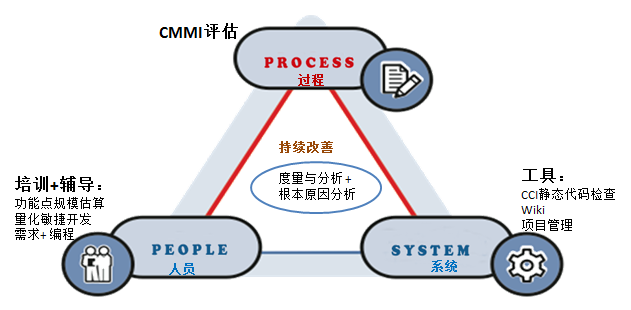
\includegraphics[width=10cm]{3个关键点图1.png}

某咨询顾问的回顾：

我们提供wiki服务器，里面除了提供模型、Q\&A问答、视频等，帮助团队了解CMMI的最佳实践。并要求每个项目组按模型的每一条实践，写出是如何在项目组体现。要顺利通过CMMI评估，项目组不仅需要提供数据，也需要参加访谈，把项目的故事讲出来。\\
因Wiki服务器是个交互平台，公司每个人都可以随时访问，所以评估组和我可以随时了解到他们对CMMI
实践的理解是否有错误。\\

\hypertarget{ux9879ux76eeux7ecfux7406ux4e0eux5927ux5bb6ux5206ux4eabux6c47ux62a5}{%
\subsubsection{项目经理与大家分享/汇报}\label{ux9879ux76eeux7ecfux7406ux4e0eux5927ux5bb6ux5206ux4eabux6c47ux62a5}}

客户完成了CMMI
V评估后，举办项目团队评估后总结会，安排了其中的3个项目团队汇报他们在过去半年，如何利用所学到的方法达到CMMI5级评估要求。
非常高兴地看到他们已经掌握了我们老师所培训的技能------利用模板从需求计算功能点，然后从功能点估算出项目工作量、测试用例数，再利用小工具测量代码质量，并且预估最终的缺陷密度等。\\
3位项目经理每人都针对以上内容发表了的1小时的演讲，分享实战心得。\\
项目团队把学到的东西用于项目中，配合度量数据，取得具体的质量提升，且达到了相应的CMMI评估要求。\\
%\href{文件:000.jpg}{500px}

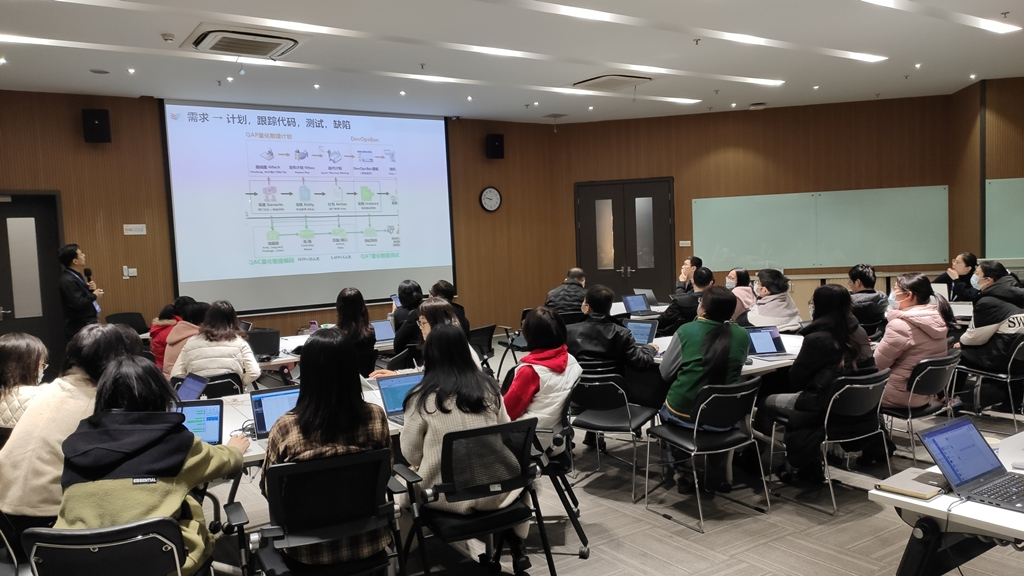
\includegraphics[width=10cm]{000.jpg}

这些项目经理都非常忙，每天可能工作到晚上10点/11点；如果没有CMMI五级评估驱动，很难在短短几个月时间内达到这效果。
其他项目组也因为听到有改进效果，产生兴趣专门抽空过来听。\\
所以若要有改进效果，大家必须把评估看成是大家学习、提升的好机会。\\
%\url{文件:3个关键点图1.png}  




